%%%%%%%%%%%%%%%%%%%%%%%%%%%%%%%%%%%%%
%%%%% PHYS305 Assignment 6
%%%%% Zachary Martin
%%%%% 5 March 2019
%%%%%%%%%%%%%%%%%%%%%%%%%%%%%%%%%%%%%

\documentclass[aps,prl,twocolumn,superscriptaddress]{revtex4-1}

\usepackage{graphicx}  % this is the up-to-date package for all figures
\graphicspath{{pictures/}} 	% Set Graphics Path
\usepackage{siunitx} % Scientific Notation and Units
\sisetup{separate-uncertainty}
\DeclareSIUnit\celeven{C^{11}}
\DeclareSIUnit\ctwelve{C^{10}}
\usepackage{amsmath, amssymb, gensymb, mathtools, bm, bigints} 	% Mathematical Tools
\usepackage{verbatim}  % for the comment environment
\usepackage{color}
% \usepackage{arydshln} % Dashed lines in table

% For inserting code snippets
\usepackage{listings}
\usepackage{xcolor}
\lstset { %
    language=C++,
    backgroundcolor=\color{black!5}, % set backgroundcolor
    basicstyle=\footnotesize,% basic font setting
}

% Shortcut Commands
\newcommand{\paren}[1]{\left( #1 \right)} 	% Parentheses for complicated expressions
\newcommand{\bparen}[1]{\left[ #1 \right]}	% Bracket parentheses for complicated expressions
\newcommand{\cmod}[1]{\left| #1 \right|}	% Mod or Absolute value

\bibliographystyle{apsrev}

% these are some custom control of the page size and margins
% \topmargin= 0.2in  % these 1st two may be needed for some computers
\textheight=9in
\textwidth=6.5in
% these next two lines give us centered text
\oddsidemargin=0cm
\evensidemargin=0cm

\begin{document}

% Title Contents
\title{PHYS 305 Assignment 6: Simulating Time Series and Isotope Decay}
\author{Zachary Martin}
\affiliation{University of Hawaii at Manoa}
\date{5 March 2019}

\begin{abstract}
We generate random data over time using programs in C++ to examine the behaviors of time series and isotope decays and how we can learn properties of the decay system from these macroscopic behaviors, that is, from bigger picture trends. We find that they exhibit a Poisson-like behavior quite accurately with measured mean within $0.22\sigma$ of the known values. From simulated isotope decays, we also find an increase in uncertainty for longer lifetimes as well as an underestimation bias in the fits. This is confirmed further in simulated decays of a sample of carbon isotopes. In C$^{11}$, the initial amount and half-life were $5.4\sigma$ and $2.2\sigma$ away from the true values, whereas the isotope C$^{10}$ with a lifetime 60x smaller resulted in measured initial amount and half-life $0.85\sigma$ and $0.05\sigma$ away from the true values. 
\end{abstract}

\maketitle

\section{Introduction and Overview}

There are various branches of physics that are dominated by probabilistic methods, such as particle physics or quantum mechanics. It is therefore important to understand how we may simulate a probability-dominated system through time using random functions in computer programs. One such example of interest is the decay of particles. Radioactive decay is a spontaneous process governed by probabilistic properties of a particle. Some of these features include the half-life or lifetime of a particle, that is, the time is takes for half of a sample of $N_0$ particles to be left or a fraction of $1/e$ to be left. The process is analogous to popcorn popping. It is random, but definitive and so once a decay has occurred, it is irreversible \cite{decay}. While the underlying process is random, we can still find macroscopic properties that many radioactive decay processes follow. We want to find these trends and use them to understand how radioactive decay works and how we can learn properties of a particle from its macroscopic trends.

\section{The Computational Problem} 
With any random system, the use of computational methods is clear. We need to simulate random decays based on a given probability or given feature of a system and generate data over many trials. 

\subsection{Time Series Decay}

\begin{figure}[htbp]
  	\begin{center}
 		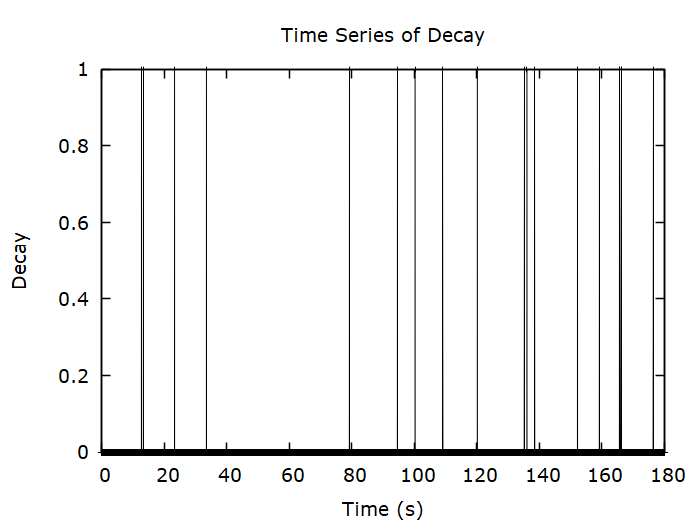
\includegraphics[scale=0.25]{tsd.png}
 		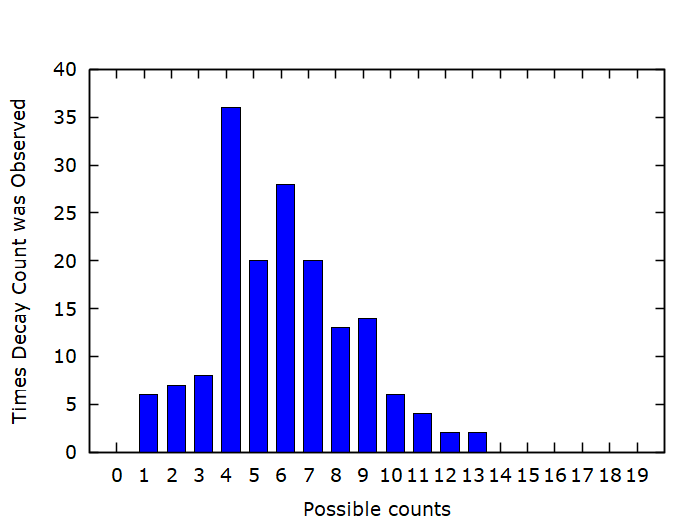
\includegraphics[scale=0.32]{tsdhisto.png}
 		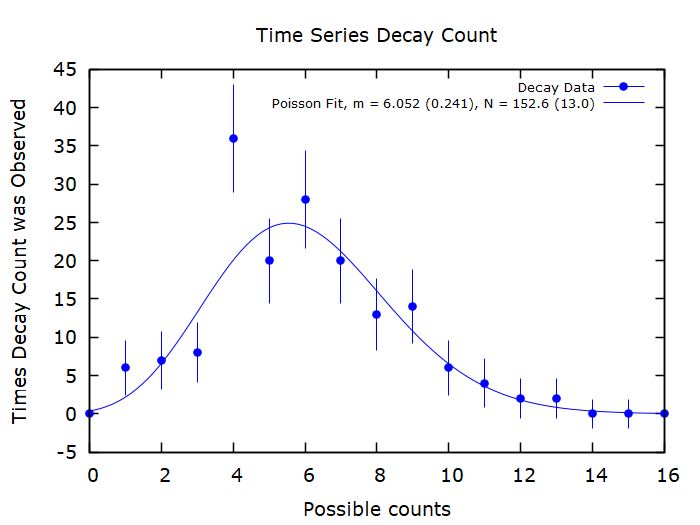
\includegraphics[scale=0.32]{tsdpois.png}
  		\caption{A simple time series of decay simulation. The top tracks each possible decay each $\SI{e-2}{\s}$. The middle shows how many minute intervals contained a certain number of decays. The last shows a Poisson distribution fit over the histogram values.}
  		\label{gr:tsd}
 	\end{center}
\end{figure}

To get a grasp on the process, we begin with a simple time series decay. A time series is a set of data using discrete time data \cite{tsd}. It is a count over certain bins, or intervals, or time. Decays are mostly governed by the decay law,
\begin{equation}
\frac{dN}{dt} = -\lambda N(t) ~, \label{eqn:declaw}
\end{equation}
where $N(t)$ is the number of particles and $\lambda$ is the decay rate. Then the decays are determined by a probability
\begin{equation}
P = \frac{\Delta N}{N(t)}~. \label{eqn:decprob}
\end{equation}
To generate decays, we simply generate a random array of numbers between 0 and 1 of the length of total points of time and ask which elements are below a given probability. If yes, then we count it as a decay. For such large numbers, we must allocate the memory using dynamic allocation methods \cite{allocation}. In the program, this looks like 
\begin{lstlisting}
double *x, *y, *m, dt=0.01; // dt in sec
int *N;
x = new double [M]();
y = new double [M]();
m = new double [200]();
N = new int [20]();
double q = .001; // probability

for (int i=0; i<M; i++){
   x[i] = drand48();
   int jminutes = i/6000;
   if (x[i] > q){
      y[i] = 0.;
   }else if (x[i] <= q){
      y[i] = 1.;
   }
   m[jminutes] += y[i];
}
\end{lstlisting}

This gives us data such as that shown in the top of Figure \ref{gr:tsd}. If we combine time data points into bins of specific length, we can count how many decays happen in each bin. Then we can sort the data in terms of how many bins contained a certain amount of decays. This results in the middle plot in Figure \ref{gr:tsd}. We can notice a Poisson distribution comes up. A Poisson distribution goes off the probability
\begin{equation}
P(\mu, k) = \mu^k \frac{e^{-\mu}}{k!}~, \label{eqn:pois}
\end{equation}
where $\mu$ is the mean and $k$ is some positive integer variable. A good estimate for the uncertainty in a Poisson distribution is
\begin{equation}
\sigma = 1 + \sqrt{N + 0.75} ~. \label{eqn:poisunc}
\end{equation}
We can fit a Poisson distribution to the binned data and find a fairly reasonable fit in the bottom of Figure \ref{gr:tsd}. Binning a million $10^{-2}$ seconds into minutes, then we get for a probability of $0.001$ that we expect about $6$ decays per minute. The Poisson fit gives a mean value of $6.052 \pm 0.421$ which is $0.22\sigma$ from the expected value, thus confirming the macroscopic behavior.

\subsection{Isotope Decay} 
We now examine a more specific application of decay simulations. Particles have a decay property called the half-life, $T_{1/2}$, or lifetime, $\tau$, which describe the time it takes for half or $1/e$ of a sample of $N_0$ particles to remain. They are related simply by \cite{Laulima}
\begin{equation}
\tau = \frac{T_{1/2}}{\log 2}~. \label{eqn:lifehalf}
\end{equation}
Using Equation \ref{eqn:declaw}, we can derive the relationships
\begin{align}
N(t) &= N_0 e^{-t/\tau} \\
N(t) &= N_0 e^{-t \log 2 / T_{1/2}} \\
\left| \frac{\Delta N}{\Delta t} \right| &= \paren{\frac{N_0 \log 2}{T_{1/2}}} e^{-t \log 2 / T_{1/2}} ~. \label{eqn:isodec}
\end{align}
Using the methods described in the Time Series Decay, we can generate decay counts over some time bins (we choose 10 s) given an initial amount and half-life, then look at the behavior over time using Equation \ref{eqn:isodec}. The code is similar:
\begin{lstlisting}
while(tt < TotalTime) {           
Ndecay = 0;  // reset decay counter

// loop over all atoms, 
// check if any decay in dt
for(int i=0;i<Nt;i++){ 
  int idecay = drand48() <= dt_DecayProb ? 
  1 : 0 ;  // conditional statement
  if(idecay){
    DecayArr[(int)(tt/bindt)] += 1.0;
    Ndecay += 1;
  }
}  
Nt -= Ndecay;
RemainArr[(int)(tt/bindt)] = Nt;

tt += dt;      
}
\end{lstlisting} 
It is possible to then fit Equation \ref{eqn:isodec} to our data and reconstruct the initial amount and half-life (and consequently the lifetime from Equation \ref{eqn:lifehalf}).

We can also do the process for a sample of multiple types of particles. For example, a sample consisting carbon isotopes C$^{10}$, C$^{11}$, C$^{12}$ may follow the decay law as
\begin{align}
\phantom{\rightarrow \left| \frac{\Delta N}{\Delta t} \right|}
&\begin{aligned}
\mathllap{N(t)} &= N_{12} + N_{11} e^{-t/T_{11}} + N_{10} e^{-t/T_{10}} 
\end{aligned} \\
&\begin{aligned}
\mathllap{\rightarrow \left| \frac{\Delta N}{\Delta t} \right|} &= \paren{N_{11} \log 2 / T_{11}} e^{-t/T_{11}} \\
&\qquad + \paren{N_{10} \log 2 / T_{10}} e^{-t/T_{10}} ~, \label{eqn:cardec}
\end{aligned}
\end{align}
where C$^{12}$ has no decay factor as it is stable. We can again use the equation above to find the half-life and initial amount, as we would with actual decay data, and then compare the results to the known values.


\section{Results and Graphs}

\begin{figure}[htbp]
  	\begin{center}
 		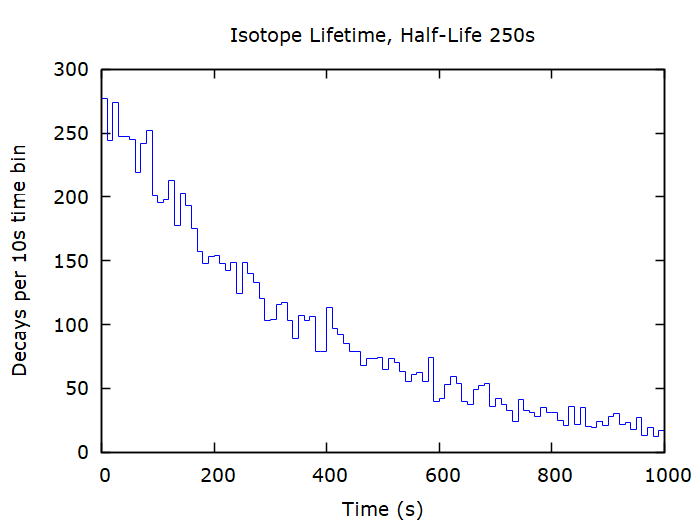
\includegraphics[scale=0.3]{step.png}
  		\caption{Discrete nature of simulated isotope decay per 10s bins.}
  		\label{gr:step}
 	\end{center}
\end{figure}

\begin{figure}[htbp]
  	\begin{center}
 		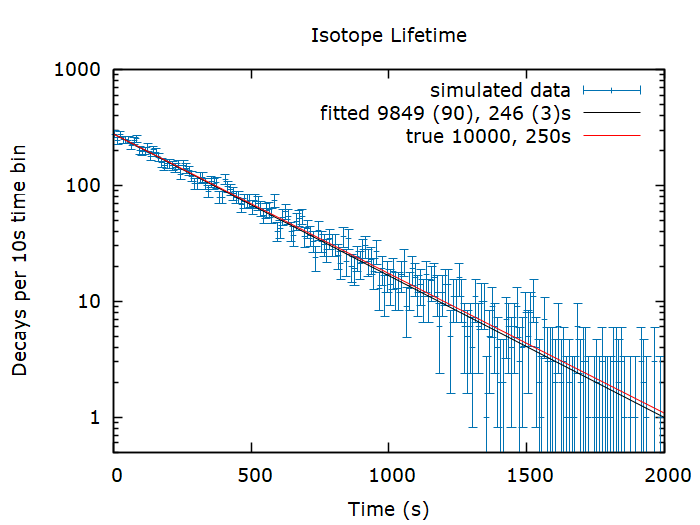
\includegraphics[scale=0.3]{iso.png}
  		\caption{Simulated isotope decay. The fit generated by Gnuplot gives a $N_0 = 9849 \pm 90$ and a half-life $T_{1/2} = \SI{246 \pm 3}{\s}$.}
  		\label{gr:iso}
 	\end{center}
\end{figure}

\begin{figure}[htbp]
  	\begin{center}
 		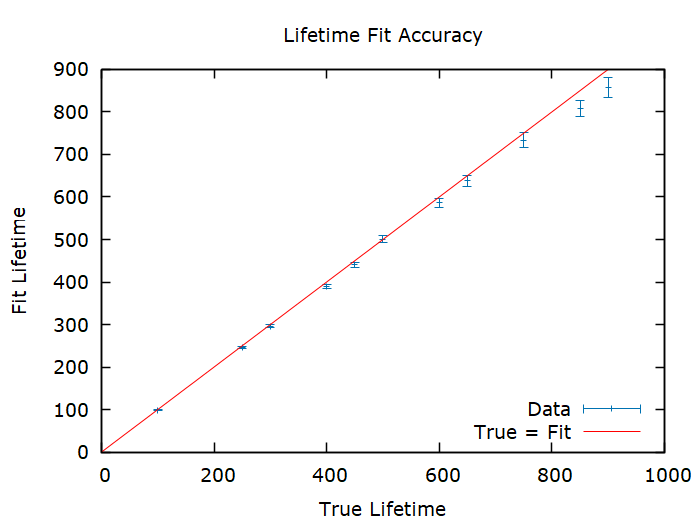
\includegraphics[scale=0.3]{ltf.png}
  		\caption{Lifetime fit comparisons for isotope decay simulations at 11 different half-lives.}
  		\label{gr:ltf}
 	\end{center}
\end{figure}

\begin{figure}[htbp]
  	\begin{center}
 		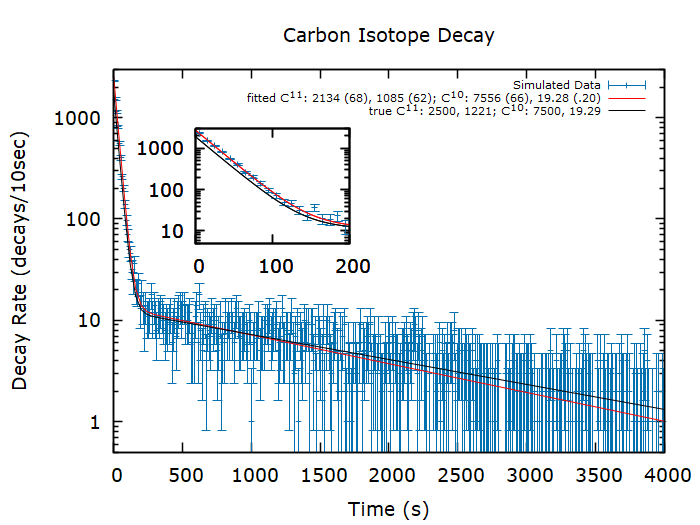
\includegraphics[scale=0.3]{isoC2.png}
  		\caption{Simulated decay rate of a sample of 10000 carbon atoms, 25$\%$ C$^{11}$ and 75$\%$ C$^{10}$ isotopes. The true half-lives of the isotopes are $T_{o, 11} = \SI{1221}{\s}$ and $T_{o, 10} = \SI{19.29}{\s}$. The fitted curve generated by Gnuplot gives the values $N_{11} = \SI{2134 \pm 68}{\celeven}$, $T_{11} = \SI{1085 \pm 62}{\s}$, $N_{10} = \SI{7556 \pm 66}{\ctwelve}$, and $T_{10} = \SI{19.28 \pm .20}{\s}$.}
  		\label{gr:carbon}
 	\end{center}
\end{figure}

\section{Discussion and Analysis}
We can see the time-discrete nature of the decay in Figure \ref{gr:step}, showing how isotope decay is a time series. We can also see an exponential behavior already just by graphing the decays per bin, which is exactly what we expect. Fitting the exponential equation \ref{eqn:isodec}, we see that it fits the data very well, especially compared to the true line. We can compare how the fits match up with the true values in Figure \ref{gr:ltf} and see that the points line up fairly well. Some things to notice is that the error seems to increase for higher lifetimes. There also seems to be a slight bias, with the points mostly being under the line, that is, the fits are underestimating the true values. I am not too sure what could be causing this.

We can see next the data for the carbon isotope decays in Figure \ref{gr:carbon}. The fits calculated initial amounts $N_{11} = \SI{2134 \pm 68}{\celeven}$, $N_{10} = \SI{7556 \pm 66}{\ctwelve}$, and half-lives $T_{11} = \SI{1085 \pm 62}{\s}$, $T_{10} = \SI{19.28 \pm .20}{\s}$. For C$^{11}$, the initial amount is $~5.4\sigma$ away, and the half-life is about $2.2\sigma$ away. For C$^{10}$, the initial amount is $~0.85\sigma$ away, and the half-life is about $0.05\sigma$ away. This is a significant difference in error between the two isotopes. This result also agrees with the Figure \ref{gr:ltf} in that the larger lifetimes do have more uncertainty. I was unable to find a good interval for binning the data that would give better results for both isotopes simultaneously. 

\section{Conclusions}
It is evident that these computational methods to analyze radioactive decays or other types of time series is useful and mostly reliable. The fluctuations can be ironed out through multiple trials of the same decay. It would seem to be difficult to obtain accurate results when examining a mix of isotopes, and so in this case it would definitely be best to do the experiments for different parameters (such as bin length) to find what works best for each isotope in question. 

Overall, this simulations has showed how we can find behaviors of random systems governed by probabilities, and analyze them to learn properties of the system. 

\section*{Acknowledgments}
\setlength{\parindent}{0cm}

\bibliographystyle{aipauth4-1}
\bibliography{bib6}



\end{document}